\chapter{Resultados}

\section{Resultados Preliminares}

Como principal resultado desse trabalho de conclusão de 
curso pode ser citado o suporte ao controlador Floodlight 
pelo Projeto RouteFlow. O Floodlight possui uma grande
comunidade de pesquisa e desenvolvimento, sendo 
amplamente utilizado em redes de larga escala. Agora será
possível aos desenvolvedores do Floodlight executarem 
experimentos usando o ambiente provido pelo Projeto
RouteFlow.

Nas seções seguintes serão mostrados testes de desempenho
 e temporização de cada um dos proxies.

\section{Testes em Ambientes Virtuais}

Todos os testes dessa seção foram feitos em um ambiente 
virtual com as seguintes configurações: computador com
processador Intel Core i7 2630QM e 6GB de memória \textit{RAM 
DDR3}. A ferramenta de virtualização escolhida foi o VMware
 Player executando uma máquina virtual com quatro núcleos 
e 1GB de memória Ram com o Ubuntu 11.04. Os testes 
mostrados abaixo foram executados para
todos os proxies do Projeto RouteFlow para que a 
virtualização tivesse o mesmo impacto sobre eles.

Para realização dos testes foi usada a ferramenta Cbench,
um software específico para testes de desempenho com 
controladores \textit{OpenFlow}. O programa basicamente
testa os controladores, gerando eventos de entrada de 
pacotes para simulação de novos fluxos. O programa emula
 um conjunto de \textit{switches} que se conectam no 
controlador, enviam pacotes de entrada (\textit{packet-in})
e aguardam a instalação de novas regras (\textit{flow-mods}).

Os proxies são desenvolvidos usando os controladores como
interface de aplicação (API). Ao testarmos o desempenho 
de um controlador acoplado ao Projeto RouteFlow estaremos
testando na verdade o desempenho do proxy propriamente 
dito. As legendas das figuras e citações abaixo fazem
referência ao controlador que serviu de interface de programação
ao proxy, ou seja, ao mencionarmos os controladores NOX,
POX ou Floodlight estamos na verdade mencionando
o proxy ao qual o controlador serviu de interface. 

A Figura \ref{fig:latencia1sw} mostra um teste com apenas
um \textit{switch} conectado. O ambiente montado pelo 
Projeto RouteFlow continha apenas uma máquina virtual
executando o software de roteamento Quagga. O teste em
questão leva em consideração uma distribuição cumulativa da
latência. Podemos notar que o desempenho do Floodlight é
parecido com o do NOX em uma grande parcela da distribuição.

\begin{figure}[h]
\centering
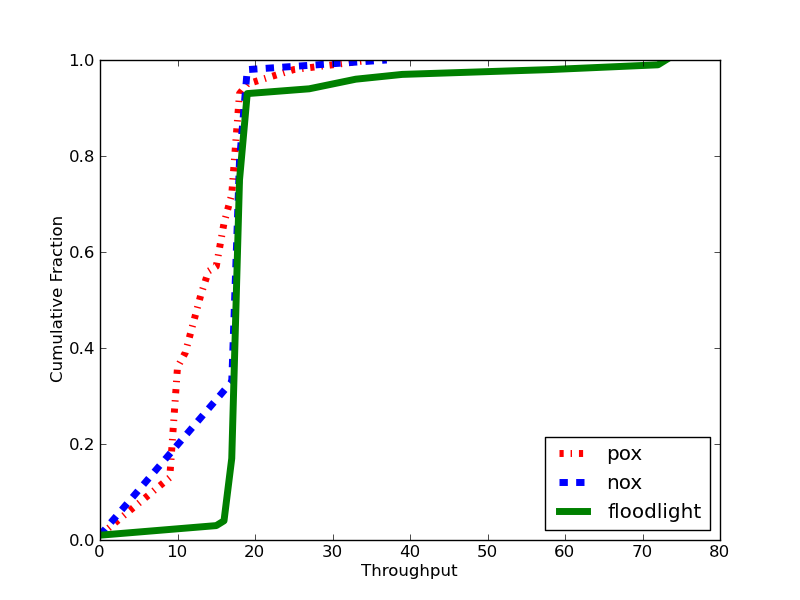
\includegraphics[width=140mm]{latencia_1sw.png}
\caption{Latência com um \textit{switch} em ms.}
\label{fig:latencia1sw} 
\end{figure}

A Figura \ref{fig:latencia4sw} foi obtida em um ambiente com
quatro \textit{switches} \textit{OpenFlow} conectados. O
ambiente RouteFlow tinha quatro máquinas virtuais executando
os algoritmos de roteamento, uma para cada \textit{switch OpenFlow}.
Isso pode ter afetado seriamente o desempenho mas, para
o âmbito do trabalho de conclusão de curso, estaremos 
testando apenas o desempenho de um proxy em relação ao
outro, sem levar em consideração o real desempenho de cada um
deles. Para termos dados reais de desempenho seria necessário
executar todos os procedimentos em um ambiente físico.
 Podemos ver
novamente que o desempenho do Floodlight é similar ao do
NOX em uma grande parcela da distribuição.

\begin{figure}[h]
\centering
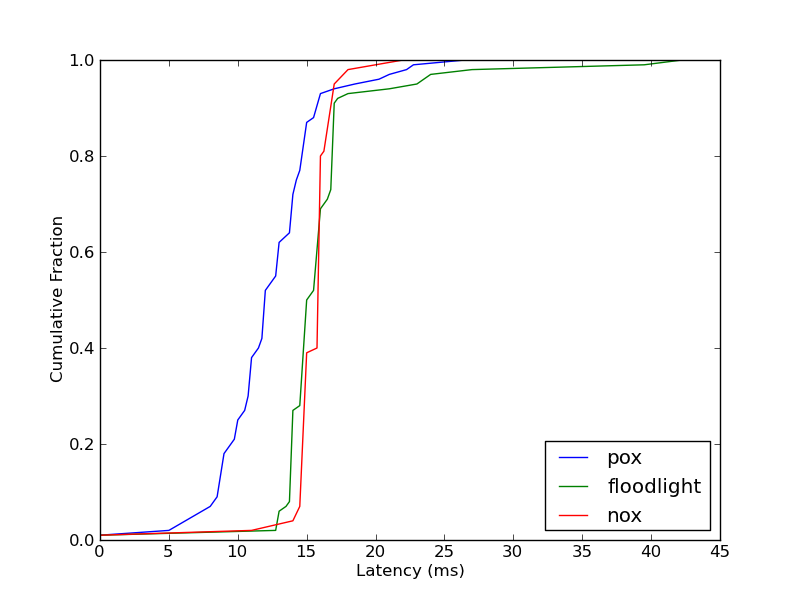
\includegraphics[width=140mm]{latencia_4sw.png}
\caption{Latência com quatro \textit{switches} em ms.}
\label{fig:latencia4sw} 
\end{figure}

Os próximos testes tratam de uma distribuição cumulativa do
desempenho do controlador em termos criação de regras por
segundo. O ambiente é o mesmo dos testes anteriores.

A Figura \ref{fig:desempenho1sw} foi obtida em um ambiente
com apenas um \textit{switch OpenFlow}. Podemos observar 
que os três controladores tiveram desempenhos semelhantes.
Tal fato pode te ocorrido devido à dupla virtualização gerada
pela linguagem Java. Novas otimizações na forma de execução
da linguagem Java poderão contribuir para o aumento do 
desempenho do Floodlight.

\begin{figure}[h]
\centering
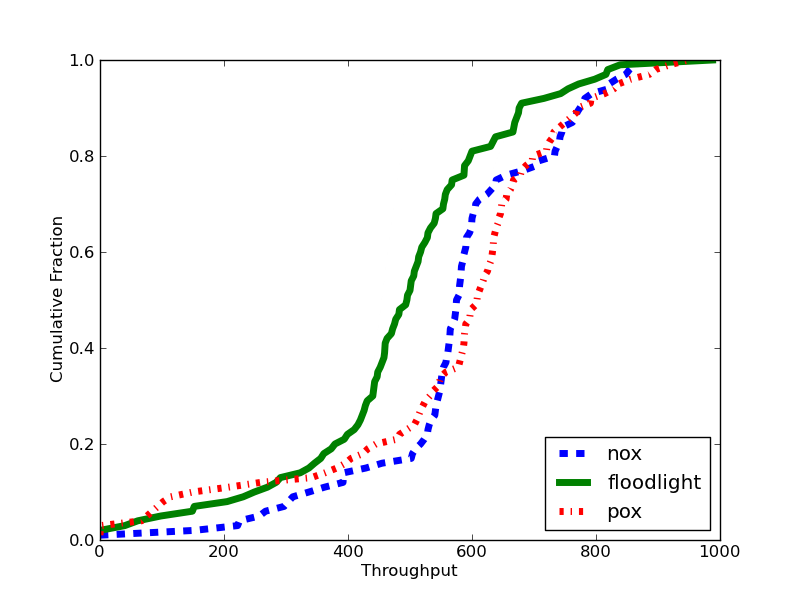
\includegraphics[width=140mm]{desempenho_1sw.png}
\caption{Desempenho com um \textit{switch} em fluxos por segundo.}
\label{fig:desempenho1sw} 
\end{figure}

A Figura \ref{fig:desempenho4sw} foi obtida em um ambiente
com quatro \textit{switches OpenFlow}. Novamente podemos
ver que o Floodlight teve desempenho parecido com o dos
outros proxies, chegando a ser mais rápido que o NOX em 
alguns momentos.


\begin{figure}[h]
\centering
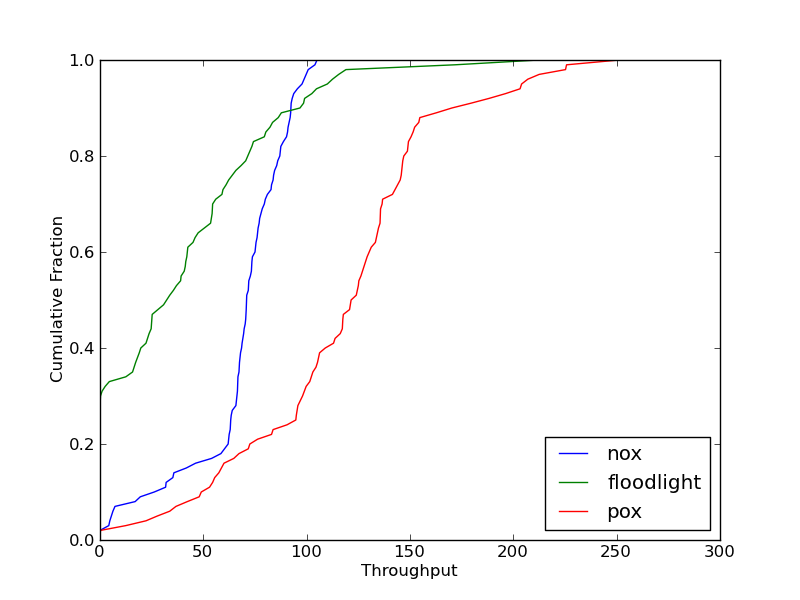
\includegraphics[width=140mm]{desempenho_4sw.png}
\caption{Desempenho com quatro \textit{switches} em fluxos por segundo.}
\label{fig:desempenho4sw} 
\end{figure}

Todos esses testes mostraram um desempenho similar entre
os três proxies levados em consideração, mostrando a viabilidade
de uso do proxy com Floodlight.

\section{Testes em Ambiente Reais}

Durante o desenvolvimento do trabalho de conclusão de
curso, um pesquisador do Departamento de Tecnologia de
Informação da Universidade Ghent (Bélgica) mostrou interesse
em usar o proxy RouteFlow com Floodlight para seus
experimentos. Parte dos experimentos foram feitos no ambiente
provido pelo Projeto OFELIA. Os experimentos
foram feitos com quatro \textit{switches OpenFlow}. Os testes
iniciais mostraram que o primeiro pacote levou cerca de 30ms
para chegar ao destino e os demais levaram cerca de
2ms, comprovando a instalação bem sucedida das regras pelo
proxy RouteFlow. O pesquisador não relatou nenhum 
problema ou inconsistência na rede, mostrando a operação
correta do proxy RouteFlow em Java.



